\documentclass[12pt,a4paper]{article}
\usepackage{../lecture-notes/vkCourseML}
\usepackage{lipsum}
\usepackage{indentfirst}
\title{Машинное обучение, ФКН ВШЭ\\Семинар №5}
\author{}
\date{}
\begin{document}
	\maketitle
	\section{AUC-ROC}
	\par На лекции мы познакомились с такой важной метрикой качества бинарной классификации, как площадь под ROC-кривой (AUC-ROC). Напомним её определение. Рассмотрим задачу бинарной классификации с метками классов $\mathbb{Y} = \{ -1, +1\},$ и пусть задан некоторый алгоритм $b(x)$, позволяющий вычислять оценку принадлежности объекта $x$ положительному классу. AUC-ROC позволяет оценивать качество классификации для семейства алгоритмов следующего вида:
	$$a(x; t) = \begin{cases}
		-1, \, b(x) \le  t,\\
		+1, \, b(x) > t,
	\end{cases}$$
	т.е. алгоритмов, присваивающих метки объектам в соответствии с оценками $b(x)$, отсекая их по некоторому порогу $t$. Каждый алгоритм (получающийся при фиксации значения порога $t$) представляется точкой на плоскости (FPR, TPR), где
	$$\text{FPR} = \frac{\text{FP}}{\text{FP}+\text{TN}} = \frac{\text{FP}}{\ell_-},$$
	$$\text{TPR} = \frac{\text{TP}}{\text{TP}+\text{FN}} = \frac{\text{TP}}{\ell_+},$$
	$\ell_-, \ell_+$ — количество объектов отрицательного и положительного классов соответственно. AUC-ROC, в свою очередь, является площадью под получившейся кривой.
	\par Изучим подробнее некоторые важные свойства данной метрики.
	
	\vspace{0.5cm}
	\par Критерий AUC-ROC имеет большое число интерпретаций — например, он равен вероятности того, что случайно выбранный положительный объект окажется позже случайно выбранного отрицательного объекта в ранжированном списке, порожденном $b(x)$. Разберем подробнее немного другую формулировку.
	
	\begin{vkProblem}
		В ранжировании часто используется функционал <<доля дефектных пар>>. Его можно определить и для задачи бинарной классификации.
	\par Пусть дан классификатор  $b(x)$, который возвращает оценки принадлежности объектов классу +1, и пусть все значения $b(x_i), \, i= \overline{1, \ell},$ для некоторой выборки $X = \{\left(x_i, y_i\right)\}_{i=1}^\ell$ различны. Отсортируем все объекты по возрастанию ответа классификатора: $b(x_{(1)}) < \dots < b(x_{(\ell)})$. Обозначим истинные ответы на этих объектах через~$y_{(1)}, \dots, y_{(\ell)}.$ Тогда доля дефектных пар записывается как
	$$\text{DP}(b, X) = \frac{2}{\ell(\ell-1)} \sum_{i < j}^\ell [y_{(i)} > y_{(j)}].$$
	Как данный функционал связан с AUC-ROC?
	\end{vkProblem}
	
	\begin{esSolution}
	Для начала разберем процедуру построения ROC-кривой. Сперва все объекты сортируются по неубыванию оценки $b(x)$, тем самым формируя список $x_{(1)}, \dots, x_{(\ell)}.$ Заметим, что для построения ROC-кривой достаточно рассмотреть\\ $(\ell+1)$ различных значений порога $t$, соответствующих всем различным способам классификации выборки, порожденным алгоритмом $b(x)$,~--- например, в качестве таких порогов можно рассмотреть следующий набор:
	\begin{align*}
		\hspace*{-5cm}&t_\ell = b(x_{(\ell)}) + 1,\\
		&t_i = \frac{b(x_{(i)}) + b(x_{(i+1)})}{2} , \, i = \overline{1, \ell -1},\\
		&t_0 = b(x_{(1)}) - 1.
	\end{align*}	
	Зафиксируем значение порога $t = t_\ell =  b(x_{(\ell)}) + 1$, в этом случае имеем
	$$\text{FPR} = \frac{\text{FP}}{\ell_-} = \frac{0}{\ell_-} = 0,$$
	$$\text{TPR} = \frac{\text{TP}}{\ell_+} = \frac{0}{\ell_+} = 0.$$
	Таким образом, алгоритму $a(x; t_\ell)$ соответствует точка (0; 0) на плоскости, откуда начинается построение ROC-кривой.
		 Будем перебирать пороги в порядке невозрастания их значения, начиная с $t_{\ell}$. Пусть мы хотим уменьшить значение порога с $t_i$ до $t_{i-1}$. При этом классификация объекта $x_{(i)}$ (и только его) изменится с отрицательной на положительную. Рассмотрим 2 случая.
	
	\begin{figure}[H]
		\center{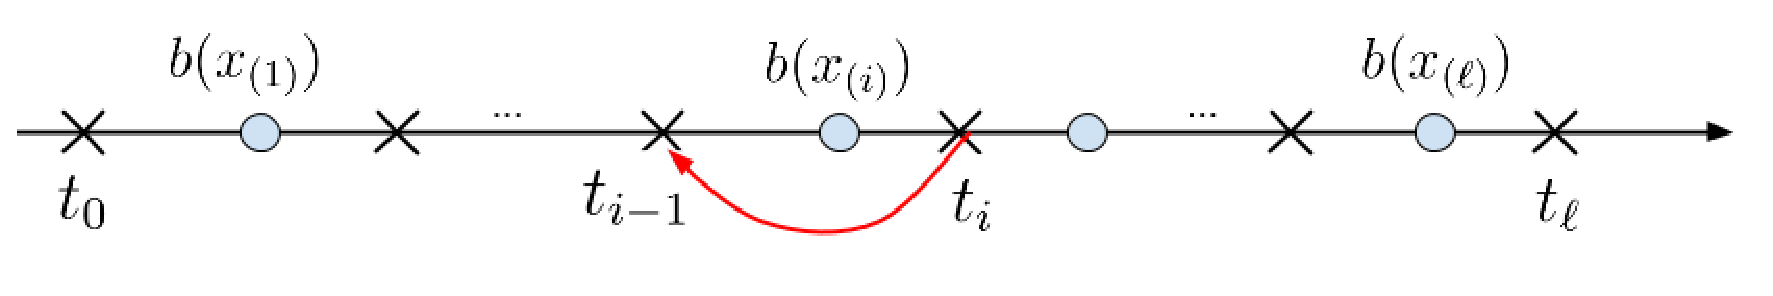
\includegraphics[width=0.8\linewidth]{./img/thresholds.eps}}
		\label{ris:image}
	\end{figure}


	\begin{enumerate}
		\item $y_{(i)} = +1.$ В этом случае классификатор начнет верно классифицировать объект, на котором ранее допускал ошибку, при этом FPR не изменится, а TPR повысится на~$\frac{1}{\ell_+}.$
		\item $y_{(i)} = -1.$ В этом случае классификатор начнет ошибаться на объекте, который ранее классифицировал верно, при этом TPR не изменится, а FPR повысится на  $\frac{1}{\ell_-}.$
	
	\end{enumerate}
	
		\begin{figure}[H]
			\center{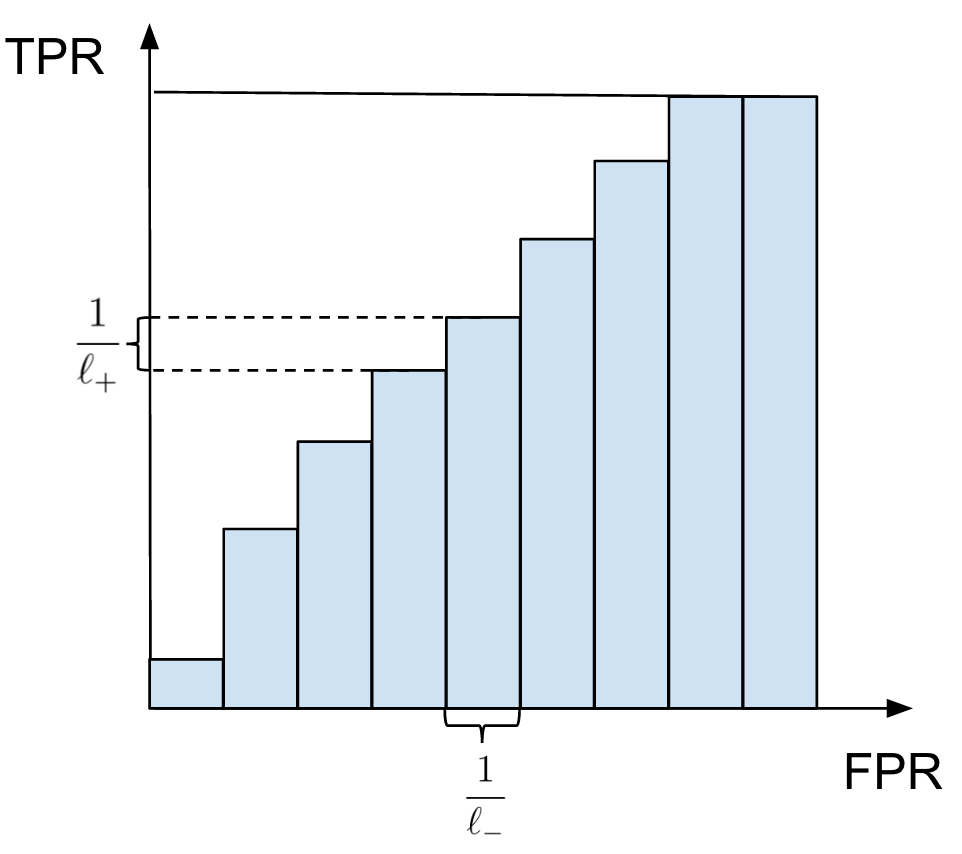
\includegraphics[width=0.6\linewidth]{./img/AUC.eps}}
			\label{ris:image}
		\end{figure}
	
	
	Теперь рассмотрим, как при этом изменяется AUC-ROC. Заметим, что область под ROC-кривой состоит из непересекающихся прямоугольников, каждый из которых снизу ограничен осью FPR, а сверху~--- одним из горизонтальных отрезков, соответствующих второму из рассмотренных случаев. Поэтому каждый раз, когда имеет место второй случай, к текущей накопленной площади под кривой (которая изначально в точке (0; 0) равна 0) добавляется площадь прямоугольника, горизонтальные стороны которого равны $\frac{1}{\ell_-}$, а вертикальные равны $\frac{1}{\ell_+} \sum_{j=i+1}^{\ell} [y_{(j)} = +1]$ (доля уже рассмотренных положительных объектов среди всех положительных), поэтому в этом случае текущее значение AUC-ROC увеличивается на $\frac{1}{\ell_- \ell_+} \sum_{j=i+1}^\ell [y_{(j)} = +1].$
	Итого, финальное значение AUC-ROC можно посчитать~следующим образом:
       \begin{align*}
      \text{AUC} &= \frac{1}{\ell_{+} \ell_{-}} \sum_{i = 1}^{\ell} [y_{(i)} = -1] \sum_{j = i + 1}^{\ell} [y_{(j)} = +1] =\\
       &= \frac{1}{\ell_{+} \ell_{-}}
        \sum_{i = 1}^{\ell} \sum_{j = i + 1}^{\ell} [y_{(i)} < y_{(j)}] =\\
        &= \frac{1}{\ell_{+} \ell_{-}} \sum_{i < j}^{\ell} (1 - [y_{(i)} = y_{(j)}] - [y_{(i)} > y_{(j)}]) =\\
        &= \frac{1}{\ell_{+} \ell_{-}} \sum_{i < j}^{\ell} (1 - [y_{(i)} = y_{(j)}]) - \frac{1}{\ell_{+} \ell_{-}} \sum_{i < j}^{\ell} [y_{(i)} > y_{(j)}] =\\
        &= \frac{1}{\ell_{+} \ell_{-}} \sum_{i < j}^{\ell} ([y_{(i)} \ne y_{(j)}]) - \frac{1}{\ell_{+} \ell_{-}} \sum_{i < j}^{\ell} [y_{(i)} > y_{(j)}] =\\
        &=
        \frac{\ell_{+} \ell_{-}}{\ell_{+} \ell_{-}}
        - \frac{1}{\ell_{+} \ell_{-}}
        \sum_{i < j}^{\ell}
        [y_{(i)} > y_{(j)}]
        = 1
        -
        \frac{1}{\ell_{+} \ell_{-}}
        \sum_{i < j}
        [y_{(i)} > y_{(j)}].
\end{align*}
	Отсюда получаем, что AUC-ROC и доля дефектных пар связаны следующим соотношением:
	$$\text{DP}(b, X) = \frac{2 \ell_- \ell_+}{\ell (\ell -1)} (1 - \text{AUC} (b, X))).$$
	\vspace{0.5cm}
	\end{esSolution}
	
	Заметим, что в случае, когда несколько объектов выборки имеют равные значения $b(x)$, при уменьшении значения порога с $t_i > b(x)$  до $t_{i-1} < b(x),$ где $x$ — один из таких объектов, изменение значений FPR и TPR происходит одновременно, поэтому  соответствующий участок ROC-кривой будет наклонным, а не горизонтальным или вертикальным.
	\begin{vkProblem}
		Пусть даны выборка~$X$, состоящая из 5 объектов, и классификатор~$b(x)$, предсказывающий оценку принадлежности объекта положительному классу. Предсказания~$b(x)$ и реальные метки объектов приведены ниже:
		\begin{align*}
		&b(x_1) = 0.2, \quad  y_1 = -1,\\
		&b(x_2) = 0.4, \quad y_2 = +1,\\
		&b(x_3) = 0.1, \quad y_3 = -1,\\
		&b(x_4) = 0.7, \quad y_4 = +1,\\
		&b(x_5) = 0.05, \quad y_5 = +1.\\
		\end{align*}
		Вычислите AUC-ROC для множества классификаторов~$a(x;t)$, порожденного~$b(x)$, на выборке~$X$.
	\end{vkProblem}
	
	\begin{esSolution}
		В соответствии с процессом построения ROC-кривой, описанным в предыдущей задаче, отсортируем оценки $b(x_i)$ в порядке их неубывания: $(b(x_{(i)}))_{i=1}^\ell = (0.05, 0.1, 0.2, 0.4, 0.7)$. Также составим последовательность реальных меток объектов из этого упорядоченного списка: $(y_{(i)})_{i=1}^\ell = (+1, -1, -1, +1, +1)$.
		
		Построим ROC-кривую (см. рис.~\ref{problem}), откуда $\text{AUC-ROC} = \frac{2}{3}$.
	\end{esSolution}
	\begin{figure}[h]
		\center{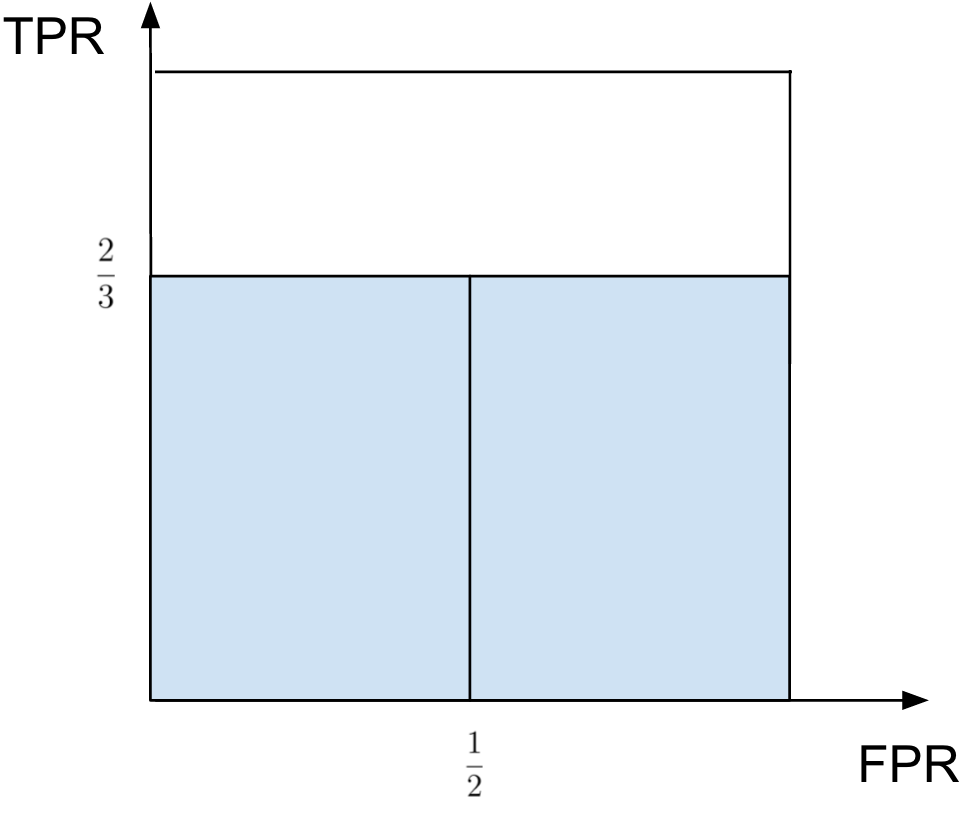
\includegraphics[width=0.4\linewidth]{./img/AUC_problem.eps}}
		\caption{Иллюстрация к задаче 1.2.}
		\label{problem}
	\end{figure}
	
	Заметим, что при вычислении AUC-ROC на некоторой выборке $X$ для итогового классификатора $a(x; t)$ важны не конкретные значения $b(x_i), \, i = \overline{1, \ell},$ а порядок расположения объектов в отсортированном по неубыванию списке $b(x_{(1)}), \dots, b(x_{(\ell)}),$ порожденным алгоритмом $b(x)$. Таким образом, для фиксированной выборки $X$ алгоритм $b(x)$ задаёт перестановку на её объектах, которая в дальнейшем используется при расчёте AUC-ROC.
	
	\vspace{0.5cm}
	
	\begin{vkProblem}
		Пусть $b(x)$ — классификатор, предсказывающий оценку принадлежности объекта $x$ классу +1 таким образом, что для некоторой выборки $X$ он равновероятно выдаёт на её объектах одну из всех возможных перестановок. Чему равно матожидание AUC-ROC этого классификатора?
	\end{vkProblem}
	
	\begin{esSolution}
	Как было показано в задаче 1.1, для AUC-ROC верно
	$$\text{AUC} = \frac{1}{\ell_{+} \ell_{-}} \sum_{i < j}^{\ell} [y_{(i)} = -1] [y_{(j)} = +1],$$
	поэтому
	$$\mathbb{E}\text{AUC} = \frac{1}{\ell_{+} \ell_{-}} \sum_{i < j}^{\ell} \mathbb{E}([y_{(i)} = -1] [y_{(j)} = +1]).$$
	Заметим, что величина $[y_{(i)} = -1] [y_{(j)} = +1]$ принимает значения 0 и 1, поэтому $$\mathbb{E}([y_{(i)} = -1] [y_{(j)} = +1]) = \mathbb{P}(y_{(i)} = -1 , \, y_{(j)} = +1) = \frac{\ell_- \ell_+ (\ell-2)!}{\ell!} = \frac{\ell_- \ell_+}{\ell (\ell-1)}.$$
	Отсюда имеем
	$$\mathbb{E}AUC = \frac{1}{\ell_- \ell_+} \sum_{i<j}^\ell \frac{\ell_- \ell_+}{\ell (\ell-1)} = 
	\frac{\ell (\ell -1)}{2} \frac{1}{\ell (\ell-1)} = \frac{1}{2}.$$
	\end{esSolution}

Итого, можем заметить, что значение AUC-ROC, близкое к $\frac{1}{2},$ означает, что классификатор близок к случайному, тогда как значение, равное 1, означает, что классификатор безошибочно классифицирует объекты при некотором значении порога.

	\begin{vkProblem}
		Пусть $b(x)$ — некоторый классификатор, предсказывающий оценку принадлежности объекта $x$ положительному классу, и при этом AUC-ROC множества классификаторов $a(x;t)$, порожденных $b(x)$, на некоторой выборке $X$ принимает значение, меньшее 0.5.
		Как можно скорректировать прогнозы классификаторов~$a(x;t)$, чтобы они были более осмысленными по сравнению с прогнозами классификатора, выдающего случайные ответы?
	\end{vkProblem}
	
	\begin{esSolution}
%		Заметим, что, поскольку $\text{AUC-ROC} < 0.5$, то ROC-кривая находится под диагональю единичного квадрата.
		
		Для некоторого классификатора $a(x;t)$ рассмотрим классификатор $a^*(x;t)$, выдающий противоположные метки по сравнению с $a(x;t)$, т.е.:
		\begin{align*}
		a^*(x;t) = -a(x;t).
		\end{align*}
		При этом TP и FP на обучающей выборке для некоторого классификатора $a^*(x;t)$ будут принимать следующие значения:
		\begin{align*}
			\text{TP}(a^*(x; t), X) = 
			\sum_{i=1}^\ell [y_i = +1]&[a^*(x;t) = +1] =\\
			&= \sum_{i=1}^\ell [y_i = +1][a(x;t) = -1] = 
			\text{FN}(a(x; t), X),\\
			\text{FP}(a^*(x; t), X) = 
			\sum_{i=1}^\ell [y_i = -1]&[a^*(x;t) = +1] =\\
			&=\sum_{i=1}^\ell [y_i = -1][a(x;t) = -1] = \text{TN}(a(x; t), X).			
		\end{align*}
		Отсюда имеем
		\begin{align*}
			\text{TPR}(a^*(x;t), X) = 
			\frac{\text{TP}(a^*(x;t), X)}{\ell_+} &= 
			\frac{\text{FN}(a(x;t), X)}{\ell_+} =\\
			&=\frac{\ell_+ - \text{TP}(a(x;t), X)}{\ell_+} 
			= 1 - \text{TPR}(a(x;t), X),\\
			\text{FPR}(a^*(x;t), X) = 
			\frac{\text{FP}(a^*(x;t), X)}{\ell_-} &= 
			\frac{\text{TN}(a(x;t), X)}{\ell_-} =\\
			&=\frac{\ell_- - \text{FP}(a(x;t), X)}{\ell_-} 
			= 1 - \text{FPR}(a(x;t), X),			
		\end{align*}
		поэтому классификатор $a^*(x;t)$ будет представлен на плоскости точкой, симметричной точке, отвечающей классификатору $a(x;t)$, относительно точки~$\left(0.5; 0.5 \right)$. 
		
		Рассмотрим ROC-кривую для множества классификаторов~$a(x;t).$ Пусть площадь областей единичного квадрата, находящихся между его диагональю и частями ROC-кривой, расположенных под ней, равна~$S_-,$ а между диагональю и частями ROC-кривой, расположенных над диагональю,~"---~$S_+.$ Тогда AUC-ROC для такой кривой принимает значение $0.5 + S_+ - S_- < 0.5$ (по условию), отсюда~$S_+ - S_- < 0.$
		
		Как было показано ранее, ROC-кривая для множества классификаторов~$a^*(x;t)$ симметрична ROC-кривой для множества классификаторов~$a(x;t),$ а потому для первой кривой область, соответствующая площади~$S_-,$ будет расположена над диагональю единичного квадрата, площади~$S_+$ "--- под диагональю. Отсюда AUC-ROC для множества классификаторов~$a^*(x;t)$ будет принимать значение $0.5 - S_+ + S_- > 0.5,$ а потому прогнозы классификаторов из этого множества  более осмысленны по сравнению со случайным классификатором.
	\end{esSolution}
	
\begin{vkProblem}\label{task:dyakonov}
На ответах алгоритма $b(x)$, отнормированных на интервал от 0 до 1, объекты отрицательного класса распределены с плотностью $p(b) = 2 - 2b,$ а объекты положительного класса распределены с плотностью $p(b) = 2b$ (см. рис. \ref{fig:densities}).
Выпишите формулу для ROC-кривой и посчитайте площадь под ней.
\end{vkProblem}

\begin{figure}[th!]
	\centering
	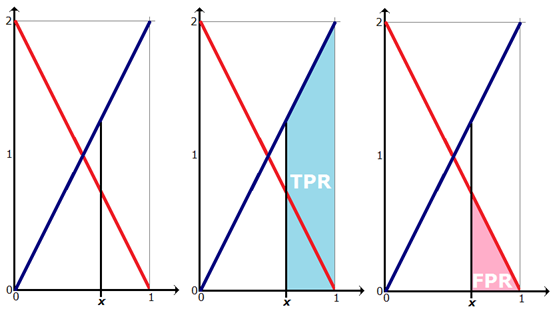
\includegraphics[width=0.5\textwidth]{./img/pic6.png}
	\caption{Распределение объектов положительного и отрицательного классов}
 \label{fig:densities}
\end{figure}

\begin{esSolution}
Для выбранного порога бинаризации $t$ значение TPR будет равно отношению площади трапеции, отсекаемой вертикальной прямой $y = t$ под синей прямой (см. рисунок) к площади всего треугольника под синей прямой.
Площадь под синей прямой равна единице (во-первых, по условию синяя прямая задаёт плотность, во-вторых, можно проверить вручную).
Площадь трапеции можно выразить как разность площадей треугольников: $TPR(t) = 1 - \frac{t \cdot 2t}{2} = 1 - t^2.$
Для FPR идея аналогичная, но нужно посчитать площадь треугольника, а не трапеции: $FPR(t) = \frac{1}{2}(1 - t)(2 - 2t) = (1 - t)^2.$
Теперь можно выразить TPR через FPR:
$TPR(t) = 1 - (1 - \sqrt{FPR(t)})^2 = 2\sqrt{FPR(t)} - FPR(t).$
Значит, ROC-кривая задаётся уравнением $y = 2\sqrt{x} - x.$
График этой кривой можно увидеть на рис. \ref{fig:roc2}.
Площадь под ней можно посчитать, взяв следующий интеграл:
$$
\int\limits_0^1 (2\sqrt{x} - x)dx = \left(\frac{4}{3}x^{\frac{3}{2}} - \frac{1}{2}x^2\right)\bigg|_0^1 = \frac{5}{6}.
$$

\begin{figure}[th!]
	\centering
	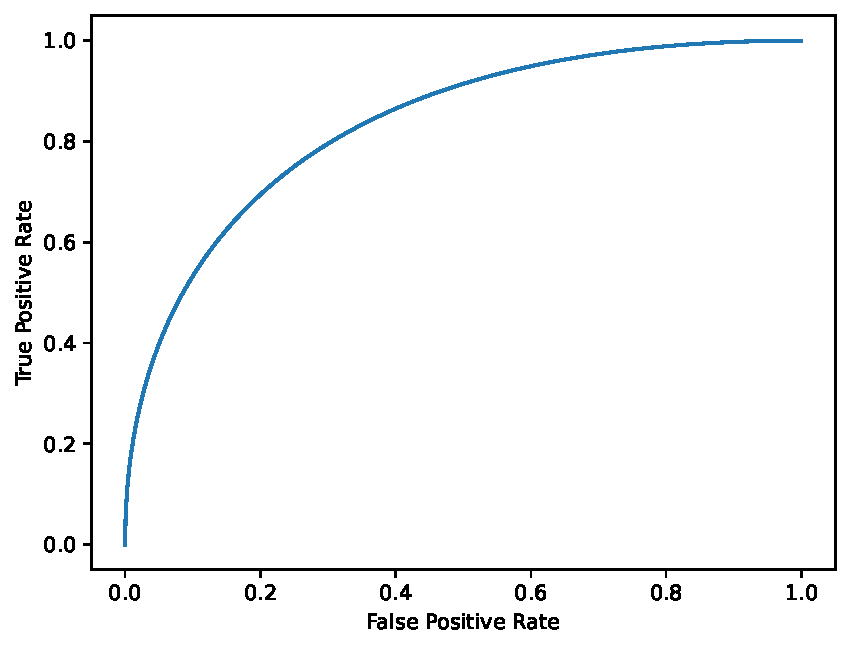
\includegraphics[width=0.5\textwidth]{./img/roc2.pdf}
	\caption{ROC-кривая из задачи \ref{task:dyakonov}}
 \label{fig:roc2}
\end{figure}

\end{esSolution}

\begin{vkProblem}
Пусть в выборке $X$ всего $\ell_{+}$ объектов положительного класса и $\ell_{-}$ объектов отрицательного класса.
Пусть $A_{xy}$ -- это множество всех перестановок элементов $X$, для которых можно выбрать порог так, чтобы получить $FP = x, FN = y.$ 
Чему равно математическое ожидание AUC ROC для классификатора, равновероятно выдающего одну из перестановок из множества $A_{xy}$?
\end{vkProblem}

\begin{esSolution}
Для AUC ROC верно
$$\text{AUC} = \frac{1}{\ell_{+} \ell_{-}} \sum_{i < j}^{\ell} [y_{(i)} = -1] [y_{(j)} = +1].$$
% Эту сумму можно переформулировать по-другому.
% Обозначим за $x_i$ выход модели на положительных объектах, за $y_i$ -- выход модели на отрицательных объектах.
% Произведение индикаторов $[y_{(i)} = -1] [y_{(j)} = +1]$ в сумме будет ненулевым, только если на более ранней $i$-ой позиции стоит отрицательный элемент, а на $j$-ой -- положительный.
% Значит, сумму можно переписать через индикатор того, что отрицательный объект стоит раньше положительного:
% $$\text{AUC} = \frac{1}{\ell_{+} \ell_{-}} \sum_{i = 1}^{\ell_{+}} \sum_{j = 1}^{\ell_{-}} [y_j < x_i].$$

Заметим, что если для перестановки возможно выбрать порог классификации, удовлетворяющий $FP = x, FN = y,$ то сделать это можно единственным способом.
Чтобы получить $FN = y,$ нам нужно иметь $TP = \ell_{+} - y;$ чтобы получить $FP = x,$ должно выполняться $TN = \ell_{-} - x.$
Значит, порог отделяет $N = \ell_{-} - x + y$ наименьших элементов от $\ell_{+} - y + x$ наибольших элементов.
Тогда разобьём сумму из выражения выше на 3 части:
\begin{enumerate}
    \item $A_1 = \sum\limits_{i \leqslant N < j}^{\ell} [y_{(i)} = -1] [y_{(j)} = +1]$ -- сумма по парам, лежащим по разные стороны от порога.
    Эту сумму легко посчитать: она равна произведению $TN \cdot TP = (\ell_{-} - x)(\ell_{+} - y).$
    \item $A_2 = \sum\limits_{i < j}^{N} [y_{(i)} = -1] [y_{(j)} = +1]$ -- сумма по парам, оба элемента в которых меньше порога (помечены моделью как отрицательные).
    Введём $1 \leqslant \alpha_1 < \ldots < \alpha_y \leqslant N$ -- позиции ложноотрицательных объектов.
    Через них эту сумму можно переписать так:
    $$A_2 = \sum\limits_{j = 2}^{N}[y_{(j)} = +1]\sum\limits_{i = 1}^{j - 1}[y_{(i)} = -1] = \sum\limits_{k = 1}^y\sum\limits_{i = 1}^{\alpha_k - 1}[y_{(i)} = -1] = \sum\limits_{k = 1}^y (\alpha_k - k) =$$
    $$=\sum\limits_{k = 1}^y \alpha_k - \frac{y(y + 1)}{2}.
    $$
    \item $A_3 = \sum\limits_{N < i < j}^{\ell} [y_{(i)} = -1] [y_{(j)} = +1]$ -- сумма по парам, оба элемента в которой больше порога (помечены моделью как положительные).
    Аналогично прошлому пункту введём $N < \beta_1 < \ldots < \beta_x \leqslant l$ -- позиции ложноположительных объектов.
    Через них эту сумму можно переписать так:
    $$
    A_3 = \sum\limits_{i = N + 1}^{\ell}[y_{(i)} = -1]\sum\limits_{j = i + 1}^{\ell}[y_{(j)} = +1] = \sum\limits_{k = 1}^x \sum\limits_{j = \beta_k + 1}^{\ell}[y_{(j)} = +1] = \sum\limits_{k = 1}^x (\ell - \beta_k - (x - k)) =
    $$
    $$
    = x(\ell - x) + \frac{x(x + 1)}{2} - \sum\limits_{k = 1}^x \beta_k = x\ell -\frac{x(x - 1)}{2} - \sum\limits_{k = 1}^x \beta_k.
    $$
\end{enumerate}
В итоге AUC можно записать так:
$$
\frac{A_1 + A_2 + A_3}{\ell_{+}\ell_{-}} = \frac{1}{\ell_{+}\ell_{-}}\left(\ell_{+}\ell_{-} + xy + \ell_{-}(x - y) - \frac{y(y + 1)}{2} - \frac{x(x - 1)}{2} + \sum\limits_{k = 1}^y \alpha_k - \sum\limits_{k = 1}^x \beta_k\right)
$$

Теперь для подсчёта математического ожидания всего выражения нам достаточно посчитать математическое ожидание $\alpha_k$ и $\beta_k$.
При фиксированном значении $\alpha_k = s$ есть $C_{s - 1}^{k - 1}$ вариантов выбрать меньшие $\alpha$ и $C_{N - s}^{y - k}$ вариантов выбрать бОльшие $\alpha$ (считаем, что если в биномиальном коэффициенте $C_n^k$ выполнено $n < k$, то он равен нулю).
Всего вариантов выбрать позиции для ложноположительных элементов -- $C_{N}^y.$
Тогда по определению математическое ожидание записывается так:
$$
\mathbb{E}\alpha_k = \frac{\sum\limits_{s = 1}^{N}sC_{s - 1}^{k - 1}C_{N - s}^{y - k}}{C_{N}^y}
$$
Выпишем математическое ожидание суммы (воспользуемся свёрткой Вандермонда):
$$
\mathbb{E}\left(\sum\limits_{k = 1}^y \alpha_k\right) = \frac{\sum\limits_{s = 1}^N s \sum\limits_{k = 1}^y C_{s - 1}^{k - 1}C_{N - s}^{y - k}}{C_{N}^y} = \frac{\sum\limits_{s = 1}^N s C_{N - 1}^{y - 1}}{C_{N}^y} = \frac{N(N + 1)}{2} \frac{(N - 1)!}{(y - 1)! (N - y)!} \frac{y! (N - y)!}{N!} =$$
$$= \frac{y(N + 1)}{2}.
$$
Для математического ожидания $\beta_k$ аналогичным способом получаем формулы:
$$
\mathbb{E}\beta_k = \frac{\sum\limits_{s = N + 1}^{\ell} s C_{s - N - 1}^{k - 1} C_{\ell - s}^{x - k}}{C_{\ell - N}^x};~~~\mathbb{E}\left(\sum\limits_{k = 1}^x \beta_k\right) = \frac{\sum\limits_{s = N + 1}^{\ell}s C_{\ell - N - 1}^{x - 1}}{C_{\ell - N}^x} = \frac{x(\ell + N + 1)}{2}.
$$
Подставим в обе формулы $N = \ell_{-} - x + y:$
$$
\mathbb{E}\left(\sum\limits_{k = 1}^y \alpha_k\right) = \frac{y(\ell_{-} - x + y + 1)}{2};~~~\mathbb{E}\left(\sum\limits_{k = 1}^x \beta_k\right) = \frac{x(\ell + \ell_{-} - x + y + 1)}{2}.
$$
Тогда при подстановке в итоговую формулу получаем
$$
\mathbb{E}\text{AUC} = \frac{1}{\ell_{+}\ell_{-}}\left(\ell_{+}\ell_{-} - \frac{1}{2}\left(y\ell_{-} + x\ell_{+}\right) \right) = 1 - \frac{1}{2}\left(\frac{y}{\ell_{+}} + \frac{x}{\ell_{-}}\right).
$$
\end{esSolution}

\begin{vkProblem} \label{task:economics}
У банка всего 4000 клиентов.
Маркетингового бюджета нового предложения банка хватит на то, чтобы обзвонить 800 клиентов.
По историческим данным аналитики банка выяснили, что лишь 6\% клиентов действительно начинают пользоваться новым предложением после маркетингового звонка.
У компании уже есть два классификатора $A$ и $B$, для которых положительный класс -- это клиенты, которые отреагируют на маркетинговый звонок, а отрицательный -- клиенты, на которых он не повлияет.
Известно, что для $A$ $FPR = 0.1, TPR = 0.2$, а для $B$ $FPR = 0.25, TPR = 0.6.$
Постройте на их основе классификатор, который выберет ровно 800 клиентов для совершения маркетинговых звонков.
\end{vkProblem}

\begin{esSolution}
Запишем условие на то, что классификатор выберет ровно 800 клиентов: $FPR \cdot \ell_{-} + TPR \cdot \ell_{+} = 800.$
Это можно представить в виде прямой, заданной в том же пространстве, что и ROC-кривая.
Чему равны $\ell_{-}$ и $\ell_{+}$ в нашем случае?
Воспользуемся данными аналитиков и получим, что среди всех клиентов будет $0.06 \cdot 4000 = 240$ клиентов, относящихся к положительному классу, и 3760 клиентов, относящихся к отрицательному классу.

Посмотрим, сколько объектов положительного класса нам выдадут классификаторы $A$ и $B$.
Для $A$: $0.1 \cdot 3760 + 0.2 \cdot 240 = 424$ -- слишком мало
Для $B$: $0.25 \cdot 3760 + 0.6 \cdot 240 = 1084$ -- слишком много.

Проведём отрезок между точками $A$ и $B$ в пространстве ROC-кривой.
Заметим, что мы можем получить любой классификатор с парой характеристик $(FPR, TPR),$ лежащей на этом отрезке.
Для этого нам достаточно брать предсказания данных двух классификаторов с вероятностями, пропорциональными расстояниям от точки до концов отрезков.

Выпишем уравнение прямой, проходящей через точки $A$ и $B$, и найдём её точку пересечения с прямой, заданной в условии.
Для прямой, проходящей через точки $A$ и $B$ верно, что 
$$
\begin{cases}
    0.2 = a \cdot 0.1 + b\\
    0.6 = a \cdot 0.25 + b
\end{cases}
\Leftrightarrow 
\begin{cases}
    b = 0.2 - a \cdot 0.1\\
    0.4 = a \cdot 0.15
\end{cases}\Leftrightarrow \begin{cases}
    a = \frac{8}{3}\\
    b = -\frac{1}{15}
\end{cases}.
$$
Значит, нам надо найти точку пересечения прямых $TPR = \frac{8}{3} \cdot FPR - \frac{1}{15}$ и $TPR = \frac{10}{3} - \frac{47}{3} \cdot FPR.$ Получаем точку $FPR = \frac{51}{275}, TPR = \frac{353}{825}.$
Осталось посчитать отношение, в котором эта точка делит отрезок:
$$\frac{\frac{51}{275} - \frac{1}{10}}{\frac{1}{4} - \frac{1}{10}} = \frac{94}{165}.$$
Значит, для получения искомого классификатора с вероятностью $\frac{94}{165} \approx 0.57$ надо брать предсказание классификатора $B$, иначе -- предсказание классификатора $A$.
Иллюстрацию к задаче можно найти на рис. \ref{fig:const}.

\begin{figure}[th!]
	\centering
	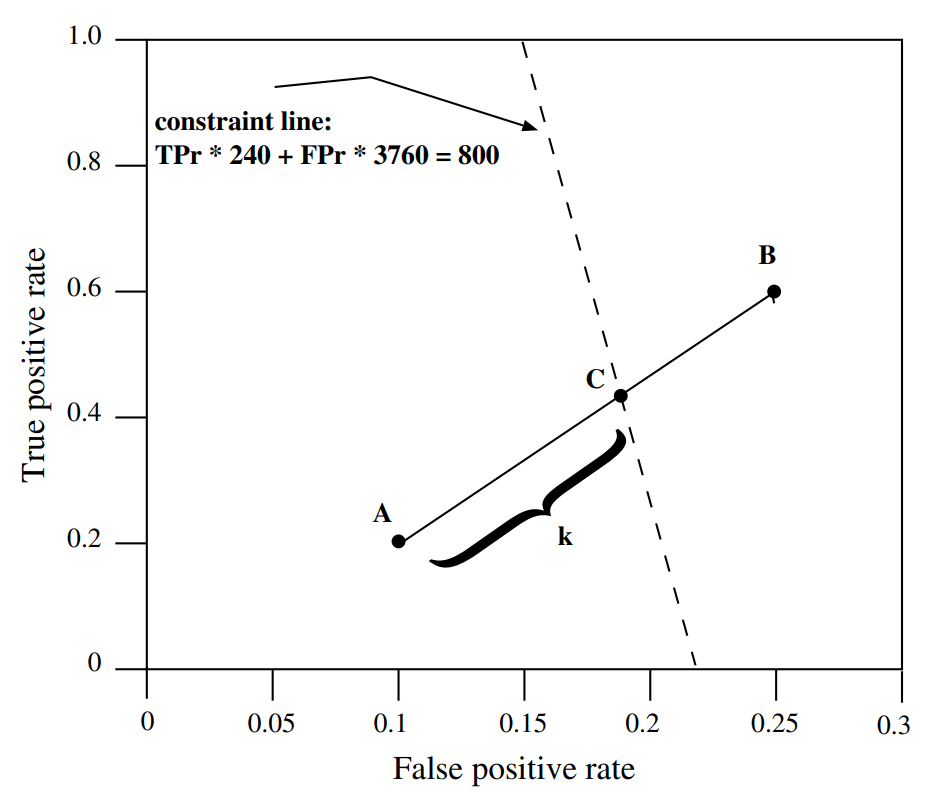
\includegraphics[width=0.5\textwidth]{./img/ml_roc_cross.png}
	\caption{Иллюстрация к задаче \ref{task:economics}.}
 \label{fig:const}
\end{figure}

\end{esSolution}

\begin{vkProblem}
Зафиксируем число объектов положительного ($\ell_{+}$) и отрицательного ($\ell_{-}$) классов.
Докажите, что ROC-кривая классификатора $A$ не ниже ROC-кривой классификатора $B$ в любой точке тогда и только тогда, когда PR-кривая классификатора $A$ не ниже PR-кривой классификатора $B$ в любой точке.
\end{vkProblem}

\begin{esSolution}
Докажем, что если ROC-кривая выше, то и PR-кривая выше.
Выберем для двух классификаторов такие пороги $t_1$ и $t_2$, что $TPR_A(t_1) = TPR_B(t_2).$
Проверим, как при этом соотносятся их точности.
Известно, что ROC-кривая $A$ выше ROC-кривой $B$, поэтому $FPR_A(t_1) \leqslant FPR_B(t_2) \Leftrightarrow FP_A(t_1) \leqslant FP_B(t_2).$
Вспомним формулу для точности: $PR_A(t) = \frac{TP_A(t)}{TP_A(t) + FP_A(t)}.$
Из условия $TPR_A(t_1) = TPR_B(t_2)$ следует равенство $TP_A(t_1) = TP_B(t_2),$ а значит, $PR_A(t_1)$ и $PR_B(t_2)$ отличаются только за счёт $FP$ в знаменателе.
Воспользовавшись полученным выше неравенством на $FP$, получаем, что $PR_A(t_1) \geqslant PR_B(t_2),$ ч.т.д.. 

Доказательство в обратную сторону проделывается абсолютно аналогично: надо зафиксировать пороги с равной полнотой и сравнить точности.
Как и в прошлом случае, точности будут отличаться только за счёт $FP$, так что из неравенства точностей мы получим неравенство для $FPR$.
\end{esSolution}

\begin{vkProblem}
	Рассмотрим задачу классификации с выборкой $X$ и долей объектов с $ y = + 1 $ равной $ 0.5 $.
	Разделим ее на две равные части: $ X_1 $ и $ X_2 $.
	Баланс классов в них равен $ p_1 $ и $ p_2 $ соответственно.
	Легко показать, что $ p_1 = 1 - p_2 $.
	
	Будем говорить, что $ X_1 $ и $ X_2 $ – это два сегмента нашей выборки.
	На них используются два разных классификатора $ a_1(x) $ и $ a_2(x) $.
	Модель на всей выборке можно записать так:
	$$
		a(x) = a_1(x)\,\left[x \in X_1\right] + a_2(x)\,\left[x \in X_2\right]
	$$
	Пусть на каждом сегменте работает случайный классификатор:
	$$
		\text{AUC}\,(a_1) = \text{AUC}\,(a_2) = 0.5
	$$
	Может ли $ \text{AUC}\,(a) $ быть больше?
	Каким может быть качество модели на всей выборке?
\end{vkProblem}

\begin{esSolution}
	Воспользуемся вероятностным определением метрики ROC AUC:
	$$
		\text{AUC}\,(a) = \mathbb P \big \{ a(x_i) > a(x_j)\; |\; y_i = +1,\; y_j = -1 \big \}
	$$
	Проведем вероятностный эксперимент: выберем случайный объект положительного класса и случайный объект отрицательного класса.
	Вероятность того, что на первом объекте ответ модели больше, и является ROC AUC модели.
	
	Рассмотрим такой вероятностный эксперимент для классификатора $ a $.
	Случайный \textit{положительный} объект принадлежит первому сегменту $ X_1 $ с вероятностью
	$$
		\dfrac{p_1}{p_1 + p_2} = \dfrac{p_1}{p_1 + 1 - p_1} = p_1
	$$
	И с вероятностью $ 1 - p_1 $ – второму сегменту, $ X_2 $.
	
	Аналогично случайный \textit{отрицательный} объект принадлежит первому сегменту $ X_1 $ с вероятностью 
	$$
		\dfrac{1 - p_1}{1 - p_1 + 1 - p_2} = \dfrac{1 - p_1}{1 - p_1 +  p_1} = 1 - p_1
	$$
	И с вероятностью $ p_1 $ – второму сегменту, $ X_2 $.
	
	Если и положительный, и отрицательный объект принадлежат $ X_1 $, то
	$$
		\mathbb{P} \left\{ a(x_i) > a(x_j)\; |\; y_i = +1,\; y_j = -1,\; x_i,\; x_j \in X_1  \right\}
		=
		\text{AUC}\,(a_1) = 0.5
	$$
	Обозначим эту вероятность $ \text{auc}_{11} $.
	Оба объекта принадлежат первому сегменту с вероятностью $ \delta_{11} = p_1 (1 - p_1) $.
	Аналогично с вероятностью $ \delta_{22} = p_1 (1 - p_1) $ оба объекта принадлежат $ X_2 $, и $ auc_{22}=0.5 $.
	
	Но что будет, если положительный объект из $ X_1 $, а отрицательный из $ X_2 $?
	Предположим, что предсказания модели на первом сегменте \textit{всегда больше} предсказаний модели на втором.
	$$
		a_1(x_i) > a_2(x_j)\quad \forall x_i \in X_1,\; x_j \in X_2
	$$
	Тогда $ \text{auc}_{12} = 1 $, и это происходит с вероятностью $ \delta_{12} = p_1 ^ 2 $.
	А с вероятностью $ \delta_{21} = (1 - p_1) ^ 2$ получим положительный объект из $ X_2 $ и отрицательный – из $ X_1 $.
	В этом случае $ \text{auc}_{21} = 0 $.
	
	Вычислим $ \text{AUC}\,(a) $ по формуле полной вероятности:
	\begin{multline*}
		\text{AUC}\,(a)
		=
		\text{auc}_{11}\,\delta_{11} + \text{auc}_{12}\,\delta_{12} + \text{auc}_{21}\,\delta_{21} + \text{auc}_{22}\,\delta_{22}
		= \\ =
		0.5 p_1(1 - p_1) + p_1^2 + 0.5 p_1(1 - p_1)
		=
		p_1
	\end{multline*}
	Получаем, что $ \text{AUC}\,(a) $ \textit{может принимать любые значения от 0 до 1}.
	
	Качество на всей выборке зависит от баланса классов на подвыборках после разбиения на сегменты.
	Если это разбиение случайно ($p_1 = p_2 = 0.5$), то и качество на всей выборке не будет отличаться от качества на отдельных сегментах.
	Если же разбиение на сегменты \textit{информативно}, то сам этот факт может усилить модель.
\end{esSolution}

	\subsection{Прямая оптимизация AUC-ROC}
	\par При обучении модели в бинарной классификации чаще всего решается задача минимизации верхней оценки функционала ошибки:
	\begin{align*}
	Q(a, X) = \frac{1}{\ell}\sum_{i=1}^\ell [a(x_i) \ne y_i] \le \frac{1}{\ell} \sum_{i=1}^\ell \tilde{L}(M_i) \to \min_w
	\end{align*}
	
	Однако иногда возникает необходимость оптимизировать более сложные метрики~"---~в частности, AUC-ROC. Напрямую оптимизировать подобные метрики не представляется возможным из-за их дискретной структуры, однако мы можем использовать трюк с верхней оценкой функционала ошибки и в этом случае. В задаче~1.1 мы показали, что AUC-ROC связан с долей дефектных пар в выборке, поэтому максимизация AUC-ROC равносильна минимизации доли дефектных пар.
	\begin{align*}
	&DP(b, X) = \frac{2}{\ell (\ell - 1)}\sum_{i < j}^\ell [y_i < y_j] [b(x_i) > b(x_j)] =\\  &\frac{2}{\ell (\ell - 1)}\sum_{i < j}^\ell  [y_i < y_j] [b(x_j) - b(x_i) < 0] \le \frac{2}{\ell (\ell - 1)}\sum_{i < j}^\ell  [y_i < y_j] \tilde{L}(b(x_j) - b(x_i)) \to \min_b
	\end{align*}
	Если верхняя оценка $\tilde{L}$ дифференцируема по параметрам модели, то можно оптимизировать такой функционал при помощи градиентных методов.

\end{document}
